%-----------------------------------------------
% Dateiname: TYPO3CMS.tex
% Autor    : Stefano Kowalke <blueduck@gmx.net>
% Lizenz   : BSD
%-----------------------------------------------
\section{TYPO3 CMS}
\label{sec:typo3cms}
\subsection{Geschichte}
\label{subsec:historyTypo3}
TYPO3 CMS ist ein \gls{wcms} und wurde von dem dänischen Programmierer Kaspar Skårhøj im Jahr 1997 zunächst für seine Kunden entwickelt - im Jahr 2000 von ihm unter der \gls{gpl2} veröffentlicht. Dadurch fand es weltweit Beachtung und erreichte eine breite Öffentlichkeit. Laut der Website T3Census\footnote{\url{http://t3census.info/}} gab es am 7. April 2014 208561 Installationen von TYPO3 CMS.
\\
\\
\begin{figure}[h!]
	\startchronology[startyear=1995, stopyear=2015]
	\chronoevent{1997}{Beginn der Entwicklung}
	\chronoevent[markdepth=45pt]{2001}{Version 3.0}
	\chronoevent{2006}{Versoin 4.0}
	\chronoevent[markdepth=25pt]{2011}{Versoin 4.5 LTS}
	\chronoevent[markdepth=55pt]{2014}{Version 6.2 LTS}
	\stopchronology
	\caption{Zeitachse der TYPO3 CMS Entwicklung}
\end{figure}

Im Jahr 2012 entschied sich das Projekt zu einer Änderung in der Namesgebung:
\begin{itemize}
	\item aus TYPO3 v4\footnote{Damit ist das von Skårhøj entwickelte \gls{cms} gemeint, welches den 4.x Zweig des Projekts darstellt.} wurde TYPO3 CMS
	\item aus FLOW3 wurde TYPO3 Flow
	\item und aus TYPO3 5.0 / TYPO3 Phoenix wurde TYPO3 Neos
\end{itemize}

Diese Änderung wurde notwendig, da schon länger abzusehen war, dass TYPO3 Phoenix nicht den Nachfolger von TYPO3 v4 darstellt. Somit war die Entwicklung von TYPO3 v4 in dem Versionszweig 4.x gefangen und es konnten keine neuen Features eingebaut oder veraltete Funktionen entfernt werden. Durch dieses neue Schema bekommt der Name "TYPO3" die Bedeutung einer Dachmarke zuteil, während "TYPO3 CMS", "TYPO3 Flow" und "TYPO3 Neos" Produkte innerhalb der TYPO3 Familie darstellen. Im weiteren Verlauf dieser Arbeit werden ausschließlich die neuen Namen verwendet.

Heute kümmert sich ein Team um die Entwicklung von TYPO3 CMS und eines um TYPO3 Flow und TYPO3 Neos. Dahinter steht keine Firma, wie es bei anderen Open Source Projekten wie Drupal (Acquia) oder Wordpress (Automattic) vorzufinden ist, sondern die \gls{t3assoc}. Die \gls{t3assoc} ist ein gemeinnütziger Verein und wurde 2004 von Kaspar Skårhøj und anderen Entwicklern gegründet um als Anlaufstelle für Spenden zu dienen, die die langfristige Entwicklung von TYPO3 sicherstellen sollen. Die Spenden werden in Form von Mitgliedsbeiträgen erhoben.\footnote{\url{http://association.typo3.org/}}

\subsection{Definition}
TYPO3 CMS ist ein klassisches \gls{cms}, welches auf die Erstellung, die Bearbeitung und das Publizieren von Inhalten im Intra- oder Internet spezialisiert ist und es somit per Definition zu einem \gls{wcms} macht.

Daneben findet man auch die Bezeichnung \gls{ecms}\footnote{\url{http://www.typo3.org}}, was als Hinweis auf den Einsatz des Systems für mittel- bis große Webprojekte dient.

Als letztes sei noch erwähnt, dass TYPO3 CMS ebenso zu den \gls{cmf} gezählt werden kann, da es dem Entwickler verschiedene \gls{api}s zur Verfügung stellt. Dieser Begriff findet sich unter anderen in einem Kommentar im – von TYPO3 CMS erzeugten – HTML-Code:
\begin{minted}[mathescape]{html}
<!--
    This website is powered by TYPO3 - inspiring people to share!
    TYPO3 is a free open source Content Management Framework
    initially created by Kasper Skaarhoj and licensed under GNU/GPL.
    TYPO3 is copyright 1998-2012 of Kasper Skaarhoj. Extensions
    are copyright of their respective owners.
    Information and contribution at http://typo3.org/
-->
\end{minted}

\subsection{Architektur und Aufbau von TYPO3 CMS}
\label{subsec:architectureTypo3}
Im folgenden werden die grundlegenden Konzepte von TYPO3 CMS vorgestellt. Dort wo es für das weitere Verständnis notwendig ist, wird tiefer in das Thema eingestiegen. Ansonsten werden die Konzepte lediglich angerissen um einen generellen Überblick zu erhalten.

\subsubsection{Webstack als Basis}

TYPO3 CMS wurde in \gls{php} - basierend auf dem Konzept der Objektorientierung - geschrieben und ist damit auf jeder Plattform lauffähig, die über einem \gls{php} Interpreter verfügt. Die Version 6.2 von TYPO3 CMS benötigt mindestens \gls{php} 5.3.7.

\gls{php} bildet zusammen mit einem Apache Webserver und einer MySQL Datenbank den sogenannten Webstack, der abhängig von dem eingesetzten Betriebssystem MAMP (OSX / {\bfseries M}ac), LAMP ({\bfseries L}inux) oder WAMP ({\bfseries W}indows) heißt.

In der Standardeinstellung kommt MySQL als Datenbank zum Einsatz - durch die Systemextension\footnote{Eine kurze Einführung in die verschiedenen Arten von Extension findet sich im Kapitel \ref{subsubsec:sysext}} \textit{DBAL} können jedoch auch Datenbanken anderer Hersteller angesprochen werden. Eine genaue Analyse dieser Extension erfolgt im Kapitel~\ref{extDBAL}[Kapitel zur Analyse von ext:DBAL einfügen].

\subsubsection{Ansichtssache}
Aus Anwendersicht teilt sich TYPO3 CMS in zwei Bereiche:

\begin{itemize}
	\item das Backend\\
		stellt die Administrationsoberfläche dar. Hier erstellen und verändern Redaktuere die Inhalte; während Administratoren das System von hier aus konfigurieren
	\item das Frontend\\
		stellt die Website dar, die ein Besucher zu Gesicht bekommt.
\end{itemize}
(vgl. \cite[S. 5]{book:dulepovTypo32008})

\subsubsection{Der Systemkern und die \gls{api}s}
\label{basics:typo3:subsubsec:coreAndApi}
TYPO3 CMS besteht aus einem Systemkern, der lediglich grundlegende Funktionen zur Datenbank-, Datei- und Benutzerverwaltung zu Verfügung stellt. Dieser Kern ist nicht monolithisch aufgebaut, sondern besteht aus Systemextensions. (vgl. \cite[S. 32]{book:laborenzTypo32006})

\begin{figure}[H]
	\centering
	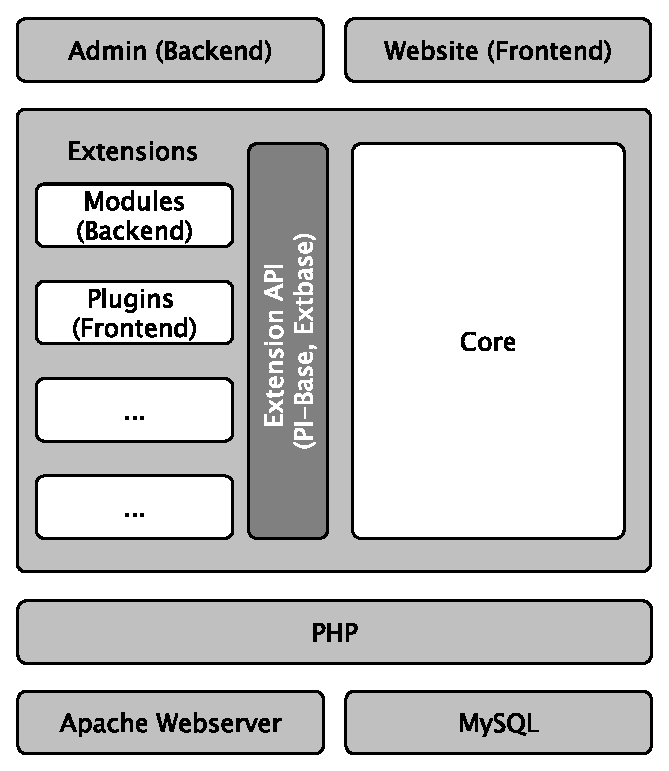
\includegraphics[scale=0.77]{diagrams/TYPO3Architecture.eps}
	\caption{Schematischer Aufbau von TYPO3}
	\label{fig:typo3Architecture}
\end{figure}

Die Gesamtheit aller von TYPO3 CMS zur Verfügung gestellten \gls{api}s, wird als die \mbox{\textit{TYPO3 API}} bezeichnet. Diese kann - analog zum Konzept von Backend und Frontend - in eine \mbox{\textit{Backend \gls{api}}} und eine \mbox{\textit{Frontend \gls{api}}} unterteilt werden kann. Die Aufgabe der Frontend \gls{api} ist die Zusammenführung der getrennt vorliegenden Bestandteile (Inhalt, Struktur und Layout) aus der Datenbank oder dem Cache zu einer HTML-Seite. Die Backend \gls{api} stellt Funktionen zur Erstellung und Bearbeitung von Inhalten zur Verfügung. (vgl. \cite[S. 5 ff.]{book:dulepovTypo32008})

Die \gls{api}s, die keiner der beiden Kategorien zugeordnet werden kann, bezeichnet Dulepov \cite[S. 5 ff.]{book:dulepovTypo32008} als \mbox{\textit{Common-\gls{api}}}. Die Funktionen der Common-\gls{api} werden von allen anderen \gls{api}s genutzt. Ein Beispiel dafür stellt die Datenbank \gls{api} dar, welche in der Regel nur einfache Funktionen wie das Erstellen, Einfügen, Aktualisieren, Löschen und Leeren\footnote{CRUD - {\bfseries C}reate, {\bfseries R}etrieve, {\bfseries U}pdate und {\bfseries D}elete} von Datensätzen bereitzustellen hat. Würde man je eine Datenbank \gls{api} für das Frontend und das Backend zur Verfügung stellen, bricht man eine wichtige Regel der Objekt-orientierten Programmierung - Don't repeat yourself. Dieser - mit hoher Wahrscheinlichkeit - redundante Code würde die Wartbarkeit des Programms verschlechtern und die Fehleranfälligkeit erhöhen.

Auf die aktuelle Datenbank-\gls{api} wird in Kapitel \ref{currentSituation}[KAPITEL zur Analyse der aktuellen Situation einfügen] näher eingegangen.

\subsubsection{Verzeichnisstruktur}

Im Gegensatz zu früheren TYPO3 CMS Versionen gibt es kein \mbox{\textit{Dummy-Package}}\footnote{Damit ist ein weitgehend leeres Paket gemeint, dass alle Dateien enthält die im Web\-root des Servers laufen sollen. Es stellt einen Container für die spätere Website dar.} mehr. Ab Version 6.2 enthält der Download lediglich den TYPO3 CMS Kern in Form des Verzeichnisses \pdf{typo3/}.

Dieses Verzeichnis ist außerhalb des Webroots abzulegen. Im Webroot ist ein Verzeichnis \pdf{www.example.com} anzulegen, in dem die Verzeichnisse \pdf{fileadmin/}, \pdf{typo3conf/}, \pdf{typo3temp/} und \pdf{uploads/} anzulegen sind. Das Verzeichnis \pdf{typo3\_src/} ist ein (Linux-)Symlink auf das Installationsverzeichnis von TYPO3 CMS und das Verzichnis \pdf{typo3/} ist ebenfalls ein Symlink, welcher über den Symlink \pdf{typo3\_src} auf \pdf{typo3} zeigt. Dieser Aufbau macht ein Update recht einfach, da lediglich der Symlink \pdf{typo3\_src} auf das Verzeichnis der neuen Version rekonfiguriert werden muss.

\begin{figure}[H]
\begin{Verbatim}[samepage=true]
.
├── Packages/
│   └── Libraries/
├── fileadmin/
├── typo3_src/ -> ../../typo3-6.2.0
├── typo3/ -> typo3_src/typo3
│   ├── contrib/
│   ├── ext/
│   ├── gfx/
│   ├── install/
│   ├── js/
│   ├── mod/
│   └── sysext/
├── typo3conf/
│   ├── ext/
│   │   ├── doctrine_dbal/
│   │   └── phpunit/
│   └── l10n/
├── typo3temp/
├── uploads/
├── media/
├── pics/
├── tf/
└── tx_phpunit/
\end{Verbatim}
\caption{Verzeichnisstruktur von TYPO3 CMS}
\label{pic:typo3FolderStructure}
\end{figure}
Im folgenden werden die einzelnen Verzeichnisse näher erklärt:

\begin{table}
	\begin{tabularx}{\textwidth}{|X|X|}
		\hline
		Verzeichnis & Erklärung\\ \hline
		Packages/Libraries/ & Dieser Ordner wurde von der von TYPO3 Flow übernommen. In einer der nächsten Versionen sollen hier die Extensions gespeichert werden. Im aktuellen Fall liegen hier externe Bibliotheken, die mit Composer\footnote{Ein Kommandozeilen Programm, um Abhängigkeiten in \gls{php} Projekten aufzulösen \url{https://getcomposer.org/}} installiert wurden, wie zum Beispiel Doctrine\\ \hline
		fileadmin/ & In diesem Ordner werden Dateien gespeichert, die über die Website erreichbar und ausgeliefert werden sollen. Dazu zählen CSS-, Image, HTML-Template- und TypoScriptdateien. Allgemein also Dateien, die vom Websitebetreiber hochgeladen werden.\\ \hline
		typo3/ & Der TYPO3 CMS Kern\\ \hline
		contrib/ & Bibliotheken von Drittanbietern\\ \hline
		contrib/ext/ & Das Verzeichnis für globale Extensions \\ \hline
		gfx/ & Jegliche Grafiken, die im Core verwendet werden \\ \hline
		gfx/install/ & Hier befand sich in früheren Versionen das Installtool. Aktuell existiert das Verzeichnis nur noch aus Kompatibilitätsgründen und wird in einer der nächsten Versionen entfernt. Das Installtool wurde als Sytemextension realisiert und ist im entsprechenden Ordner unter \pdf{sysext/install/} zu finden\\ \hline
		gfx/js/ & Hier befinden sich die JavaScript Bibliotheken, die von Core genutzt werden.\\ \hline
		gfx/mod/ & Enthält die Konfiguration der Hauptmodule des Backends (File, Help, System, Tools, User, Web).\\ \hline
		sysext/ & Enthält die Systemextensions.\\ \hline
		typo3conf/ & Lokale Extensions und die lokale Konfiguration\\ \hline
		typo3temp/ & Temporäre Dateien\\ \hline
		uploads/ & Dateien die vom Websitebesucher hochgeladen werden - zum Beispiel über ein Formular.\\ \hline
	\end{tabularx}
	\caption{Erläuterung der Verzeichnisstruktur von TYPO3 CMS}
	\label{tab:typo3FolderStructure}
\end{table}
Im Verzeichnis \pdf{www.example.com} muss noch ein Symlink \pdf{index.php} angelegt werden, welcher auf \pdf{typo3\_src/index.php} zeigt.

Unter \pdf{www.example.com/typo3conf/} befindet sich die Datei \pdf{LocalConfiguration.php}. Diese enthält die Grundkonfiguration in Form eines Arrays. Darin sind verschiedenen Einstellungen festgelegt:
\begin{itemize}
	\item Debug Mode
	\item Sicherheitslevel für den Login (Fronend und Backend)
	\item das Passwort für das Installtool (mit MD5 und Salt gehasht)
	\item die Zugangsdaten zur Datenbank (Benutzername, Password, Datenbankname, Socket, …)
	\item Einstellungen zum Caching
	\item Titel der Website
	\item Einstellungen zum Erzeugen von Graphiken
\end{itemize}

Die Einstellungen zur Datenbank werden im praktischen Teil näher beleuchtet.

\subsubsection{TCA}

Wie bereits geschrieben wurde, stellt das \gls{be} eine Ansicht auf die Datenbank dar. Die Inhalte werden dabei mittels Formulare eingegeben und in der Datenbank gespeichert. Die Konfiguration dieser Formulare erfolgt über ein globales \gls{php}-Array - dem \gls{tca}.

Über das TCA werden die Metadaten einer Tabelle (Datentyp, Länge, Engine) mit weiteren Daten angereichert. So können mit dem \gls{tca}

\begin{itemize}
	\itemsep1pt\parskip0pt\parsep0pt
	\item
		die Beziehungen einer Tabelle zu anderen Tabellen beschrieben werden
	\item
		in welchem Layout soll ein Feld im Formular dargestellt werden
	\item
		und wie soll das Feld validiert werden.
\end{itemize}

Enthält eine Tabelle keinen Eintrag im TCA ist sie im Backend nicht sichtbar.(vgl. \cite{web:typo3TCA})

[HINWEIS: Vielleicht kann das TCA auch einfach im Glossar beschrieben werden. Einen Eintrag gibt es schon unter tcag]

\subsubsection{XCLASS}
TYPO3 CMS besitzt einen Mechanismus, der es erlaubt Klassen zu erweitern oder Methoden mit eigenem Code zu überschreiben. Dies funktioniert für den Systemkern wie auch für andere Extensions. Dieses Feature nennt sich XCLASS und wird vom Prototypen eingesetzt um die Datenbankklasse von TYPO3 CMS zu überschreiben. Darauf wird im Kapitel [KAPITEL Analyse Ist-Zustand einfügen] näher eingegangen. Hier soll lediglich der Hintergrund zu XCLASS beschrieben werden.

Damit eine Klasse per XCLASS erweiterbar ist, darf sie nicht per \phpinline{new()} Operator erzeugt werden, sondern mit der von TYPO3 CMS angebotenen Methode\\
\phpinline{\TYPO3\CMS\Core\Utility\GeneralUtility::makeInstance()}.
Diese Methode sucht im globalen \gls{php}-Array \phpinline{$GLOBALS['TYPO3_CONF_VARS']['SYS']['Objects']} nach angemeldeten Klassen, instanziiert diese und liefert sie anstelle der Originalklasse zurück. Dieses Array dient der Verwaltung der zu überschreibenden Klassen und erfolgt in der Datei \pdf{ext\_localconf.php} innerhalb des Extensionsverzeichnisses\footnote{Zur Erläuterung des Aufbaues einer Extension siehe Kapitel~\ref{tab:extensionFolderStructure}.}.

%\begin{phpcode}
%$GLOBALS['TYPO3\_CONF\_VARS']['SYS']['Objects']['TYPO3\\CMS\\Backend\\Controller\\NewRecordController'] = array(
%'className' => 'Documentation\\Examples\\Xclass\\NewRecordController'
%);
%\end{phpcode}

Der Mechanismus hat jedoch ein paar Einschränkungen:

\begin{itemize}
	\itemsep1pt\parskip0pt\parsep0pt
	\item
		der Code der Originalklasse kann sich ändern. Es ist somit nicht sichergestellt, dass der überschreibende Code weiterhin das macht, wofür gedacht war
	\item
		XCLASSes funktioneren nicht mit statischen Klassen, statischen Methoden und finalen Klassen
	\item
		eine Originalklasse kann nur einmal per XCLASS übeschrieben werden
	\item
		einige Klassen werden sehr früh bei der Initialisierung des System instanziiert. Das kann dazu führen, dass Klassen die als Singleton ausgeführt sind, nicht überschrieben werden können oder es kann zu unvorhergesehenen Nebeneffekten kommen.
\end{itemize}

\subsection{Extensions}
Extensions sind funktionale Erweiterungen. Sie interagieren mit dem Systemkern über die Extension API und stellen die Möglichkeit dar TYPO3 CMS zu erweitern und anzupassen.

Extensions werden - je nach Kontext - in unterschiedliche Kategorien eingeteilt, die hier kurz vorgestellt werden.

\subsubsection{Einteilung}
\label{subsubsec:sysext}
Systemextension werden mit dem System mitgeliefert und befinden sich ausschließlich im Ordner \pdf{typo3/sysext/}. Sie werden nochmals unterteilt in jene, die für den Betrieb von TYPO3 CMS unabdingbar sind und solche die nicht zwangsläufig installiert sein müssen, jedoch wichtige Funktionen beisteuern. Die Extension DBAL ist in die letzte Kategorie einzuordnen. Auf sie wird im Kapitel \ref{extDBAL} näher eingegangen.

Neben Systemextensions gibt es noch globale\footnote{Da globale Extensions nur in bestimmten Szenarien einen Sinn ergeben und in der Realität so gut wie nicht vorkommen, wird von der TYPO3 Community der Begriff "Extension" synonym zum Begriff "lokale Extension" verwendet. Die Arbeit folgt dieser Regelung.} und lokale Extensions. Lokale Extensions werden im Ordner \pdf{typo3conf/ext/} und globale Extensions im Ordner \pdf{typo3/ext} installiert.

Eine weitere Kategorisierung erfolgt nach dem Aufgabengebiet einer Extension. Die Festlegung auf eine der folgenden Kategorien hat keine direkte Auswirkung auf die Funktion der Extension. Sie wird von TYPO3 CMS hauptsächlich als Sortiermerkmal im \gls{em} genutzt.

[Ich denken diese Übersicht kann gelöscht werden, da irrelevant]
\begin{itemize}
	\item
		Frontend
	\item
		Frontend Plugins
	\item
		Backend
	\item
		Backend Modul
	\item
		Service
	\item
		Example
	\item
		Templates
	\item
		Documentation
	\item
		Verschiedenens
\end{itemize}

\subsubsection{Extension Manager}
Der \gls{em} ist ein \gls{be} Modul, über das die Extensions verwaltet werden können. Es erlaubt die Aktivierung, Deaktivierung, Herunterladen und das Löschen von Extensions. Darüberhinaus bietet der \gls{em} Möglichkeiten zur detailierten Anzeige von Informationen über die Extensions wie das Changelog\footnote{Das Protokoll der Codeänderungen, die ein Programm im Laufe seines Lebens erlebt}, Angaben zu den Autoren und Ansicht der Dateien der Extension.

\subsubsection{Verzeichnisstruktur}
Unabhängig von der Einteilung der Extensions in die veschiedenen Kategorien unterscheiden sie sich nicht in der Verzeichnis- und Dateistruktur. Mit der Integration von Extbase in TYPO3 CMS hat sich eine neue Verzeichnisstruktur etabliert. Sie folgt dem Paradigma \textit{Konvention statt Konfiguration}, was bedeutet, dass durch Einhaltung der Struktur keine weitere Konfiguration notwendig ist.

[Beschreibung der Verzeichnisstruktur einfügen]

\begin{figure}[t]
\begin{Verbatim}[samepage=true]
.
├── Classes/
│   ├── Install/
│   ├── Loggers/
│   └── Persistence/
├── Configuration/
│   ├── ExtensionBuilder/
│   ├── TCA/
│   └── TypoScript/
├── Documentation/
├── Resources/
│   ├── Private/
│   └── Public/
├── Tests/
│   ├── Build/
│   └── Unit/
├── vendor/
│   ├── bin/
│   ├── composer/
│   ├── doctrine/
│   └── symfony/
├── composer.json
├── ext_emconf.php
├── ext_icon.gif
├── ext_localconf.php
├── ext_tables.php
├── ext_tables.sql
└── ext_tables_static+adt.sql
\end{Verbatim}
\caption{Verzeichnisstruktur einer Extension}
\label{pic:extensionFolderStructure}
\end{figure}
%\begin{sidewaystable}
%\begin{tabularx}{\textwidth}{|X|X|}
%\centering
\pagebreak
\begin{longtable}{|l|p{.60\textwidth}|}
	\hline
	Verzeichnis / Datei & Erklärung \\ \hline
	Classes/ & Hier erwartet TYPO3 CMS alle Klassendateien. Diese können in weiteren Unterverzeichnissen nach ihren Zweck unterteilt werden (Controller, Service, Loggers, Persistence)\\ \hline
	Configuration/ & Enthält Konfigurationsdateien wie TypoScript oder TCA.\\ \hline
	Documentation/ & Enthält die Dokumentation im ReST\footnote{reStructuredText \url{http://docutils.sourceforge.net/rst.html}} Format aus der HTML und ein PDF generiert werden kann.\\ \hline
	Resources/Private/ & Enthält die Fluid-Template\footnote{TYPO3s Templating Sprache}, Sprach- und Sassdateien. Kurz alle Dateien, die für die Struktur und das Aussehen einer Website notwendig sind, jedoch lediglich Templates darstellen und noch verarbeitet werden müssen\\ \hline
	Resources/Public/ & Hier liegen Grafiken, CSS- und Javasciptdateien\\ \hline
	Tests/ & Hier werden die PHPUnit-, Akzeptanz- und/oder Verhaltenstests abgelegt.\\ \hline
	vendor/ & Dieses Verzeichnis wird von Composer angelegt und enthält externe Abhängigkeiten wie in dem Fall Doctrine \gls{dbal}. Im Moment ist dies redunant, da der selbe Inhalt auch im Webroot der Site unter \pdf{Packages/Libraries/} verfügbar sein muss. Das liegt an der noch nicht vollständig umgesetzten Kompatibilität von TYPO3 CMS zu Composer, die jedoch in einer späteren Version noch nachgereicht wird.\\ \hline
	composer.json & Seit Version 6.2 von TYPO3 CMS ist eine Composer.json erforderlich. In ihr werden Metadaten der Extensions wie Name, Typ (System- oder lokale Extension), Lizenz, Version und Abhängigkeiten definiert. Sie wird in Zukunft wahrscheinleich die Datei \pdf{ext\_emconf.php} ablösen.\\  \hline
	ext\_emconf.php & Diese Datei ist unabdinglich für die Funktionsweise der Extensions. Sie definiert ebenso wie die \pdf{composer.json} Metadaten jedoch in einem \gls{php}-Array und nicht im JSON-Format\footnote{\url{http://json.org/}}. Diese Datei existiert seit den Anfängen von TYPO3 CMS und wird wahrscheinlich bald von der composer.json abgelöst werden.\\ \hline
	ext\_icon.gif & Ein Icon für die Extension, welches im \gls{be} angezeigt wird\\ \hline
	ext\_localconf.php & In dieser Datei wird die Extension für einen Hook oder eine XCLASS registiert.\\ \hline
	ext\_tables.php & Die Datei hat drei Aufgaben:
	\begin{itemize}
	\item Definition von Extensionstabellen
	\item Definition von Feldern und Tabellen, die von dieser Extension erweitert werden
	\item \gls{fe} Plugins und \gls{be} Module werden hier registiert
	\end{itemize}
	\\ \hline
	ext\_tables.sql & Diese Datei enthält Anweisungen um eine Datenbanktabelle zu erstellen. Sie sind im MySQL Format zu formulieren, auch wenn als Datenbank etwas anderes genutzt wird. TYPO3 CMS parst die Datei mit einem eigenen (sehr rudimentären) SQL-Parser und generiert einen eigene SQL-Abfrage. Dieses Vorgehen hat den Hintergrund, dass dadurch auf Fehler im diesen Dateien reagiert werden kann und zum anderen das die mitgelieferte Datenbankabstraktionsschicht die Anweisungen in das SQL der entsprechenden Hersteller übersetzen kann. Auf dem Inhalt dieser Datei wird im praktischen Teil in Kaptitel~\ref{subsec:extTables} noch genauer eingegangen.\\ \hline
	ext\_tables\_static+adt.sql & Auch diese Datei enthält SQL Code wie \pdf{ext\_tables.sql}. Der Unterschied besteht darin, dass sie \pdf{INSERT} Statements enhalten kann um statische Daten in eine Tabelle bei der Installation einer Extensions einzufügen. Als Beispiel sei hier der \gls{em} genannt, in dessen Tabelle wird über diese Datei die URL zum \gls{ter} eingefügt. Auf dem Inhalt dieser Datei wird im praktischen Teil in Kaptitel~\ref{subsec:extTables} noch genauer eingegangen.\\ \hline
	\caption{Erläuterung der Verzeichnisstruktur einer Extension}
	\label{tab:extensionFolderStructure}
\end{longtable}
